\documentclass[12pt]{book}

\newcommand{\thetitle}{Think Java: How to Think Like a Computer Scientist}
\title{\thetitle}

\newcommand{\theauthors}{Allen Downey and Chris Mayfield}
\author{\theauthors}

\newcommand{\theversion}{Version 6.0 Draft -- \today}
\date{\theversion}

\usepackage{geometry}
\geometry{
    width=5.5in,
    height=8.5in,
    hmarginratio=3:2,
    vmarginratio=1:1,
    includehead=true,
    headheight=15pt
}

% paragraph spacing
\setlength{\parindent}{0pt}                      % 17.62482pt
\setlength{\parskip}{12pt plus 4pt minus 4pt}    % 0.0pt plus 1.0pt
\linespread{1.05}
\def\arraystretch{1.5}

% list spacing
\setlength{\topsep}{5pt plus 2pt minus 3pt}      % 10.0pt plus 4.0pt minus 6.0pt
\setlength{\partopsep}{-6pt plus 2pt minus 2pt}  %  3.0pt plus 2.0pt minus 2.0pt
\setlength{\itemsep}{0pt}                        %  5.0pt plus 2.5pt minus 1.0pt

% these are copied from tex/latex/base/book.cls
% all I changed is afterskip
\makeatletter
\renewcommand{\section}{\@startsection {section}{1}{\z@}%
    {-3.5ex \@plus -1ex \@minus -.2ex}%
    {0.7ex \@plus.2ex}%
    {\normalfont\Large\bfseries}}
\renewcommand\subsection{\@startsection{subsection}{2}{\z@}%
    {-3.25ex\@plus -1ex \@minus -.2ex}%
    {0.3ex \@plus .2ex}%
    {\normalfont\large\bfseries}}
\renewcommand\subsubsection{\@startsection{subsubsection}{3}{\z@}%
    {-3.25ex\@plus -1ex \@minus -.2ex}%
    {0.3ex \@plus .2ex}%
    {\normalfont\normalsize\bfseries}}
\makeatother

% table of contents vertical spacing
\usepackage{tocloft}
\setlength\cftparskip{8pt plus 4pt minus 4pt}

% The following line adds a little extra space to the column
% in which the Section numbers appear in the table of contents
\makeatletter
\renewcommand{\l@section}{\@dottedtocline{1}{1.5em}{3.0em}}
\makeatother

% customize page headers
\usepackage{fancyhdr}
\pagestyle{fancyplain}
\renewcommand{\chaptermark}[1]{\markboth{Chapter \thechapter ~~ #1}{}}
\renewcommand{\sectionmark}[1]{\markright{\thesection ~~ #1}}
\lhead[\fancyplain{}{\bfseries\thepage}]%
      {\fancyplain{}{\bfseries\rightmark}}
\rhead[\fancyplain{}{\bfseries\leftmark}]%
      {\fancyplain{}{\bfseries\thepage}}
\cfoot{}
%\rfoot{\textcolor{gray}{\tiny ThinkJava Draft \today}}

% balanced index with TOC entry
\usepackage{makeidx}
\makeindex
%\usepackage[totoc]{idxlayout}

% automatically index glossary terms
\newcommand{\term}[1]{%
\index{#1}
\item[#1:]}
% TODO: doesn't work with plastex
%\newcommand{\term}[1]{\item[#1:]}

% where to find graphics
\usepackage{graphicx}
%\graphicspath{{figs/}}

%% tweak spacing of figures and captions
%\usepackage{floatrow}
%\usepackage{caption}
%\captionsetup{
%    font=small,
%    labelformat=empty,
%    justification=centering,
%    skip=4pt
%}

% format end of chapter excercises
\usepackage{amsmath}
\usepackage{amsthm}
\newtheoremstyle{exercise}
  {12pt}        % space above
  {12pt}        % space below
  {}            % body font
  {}            % indent amount
  {\bfseries}   % head font
  {}            % punctuation
  {12pt}        % head space
  {}            % custom head
\theoremstyle{exercise}
\newtheorem{exercise}{Exercise}[chapter]

% colors for code listings and output
\usepackage{xcolor}
\definecolor{bgcolor}{HTML}{FAFAFA}
\definecolor{comment}{HTML}{007C00}
\definecolor{keyword}{HTML}{0000FF}
\definecolor{strings}{HTML}{B20000}

% syntax highlighting in code listings
\usepackage{textcomp}
\usepackage{listings}
\lstset{
    language=java,
    basicstyle=\ttfamily,
    backgroundcolor=\color{bgcolor},
    commentstyle=\color{comment},
    keywordstyle=\color{keyword},
    stringstyle=\color{strings},
    columns=fullflexible,
    keepspaces=true,
    showstringspaces=false,
    upquote=true,
    aboveskip=\parskip,
    belowskip=\parskip
}

% code listing environments
\lstnewenvironment{code}
{\minipage{\linewidth}}
{\endminipage}
\lstnewenvironment{stdout}
{\lstset{commentstyle=,keywordstyle=,stringstyle=}\minipage{\linewidth}}
{\endminipage}

% pdf hyperlinks, table of contents, and document properties
\usepackage[pdftex]{hyperref}
\hypersetup{%
  pdftitle={\thetitle},
  pdfauthor={\theauthors},
  pdfsubject={\theversion},
  pdfkeywords={},
  bookmarksopen=false,
  colorlinks=true,
  citecolor=black,
  filecolor=black,
  linkcolor=black,
  urlcolor=blue
}

% inline syntax formatting
\newcommand{\java}[1]{\lstinline{#1}} %\end{
%\newcommand{\java}[1]{\verb"#1"}
%\newcommand{\java}[1]{{\tt #1}}

\begin{document}
\setcounter{chapter}{9}


\chapter{User-defined types}

\index{object type}
\index{type!object}

Way back in Section~\ref{sec:hello} when we defined the class \java{Hello}, we created a data type named \java{Hello}.
We didn't declare any variables with type \java{Hello}, and we didn't use \java{new} to create any \java{Hello} objects---but we could have!
There was no reason to create a \java{Hello} object, and it wouldn't have done much if we did.

\index{class definition}

In this chapter, we will look at defining class that create {\em useful} object types.
Here are the most important ideas:

\begin{itemize}

\item Defining a new class also creates a new object type with the same name.

\index{instance}

\item Every object belongs to some object type; that is, it is an {\bf instance} of some class.

\item A class definition is like a template for objects: it determines what attributes the objects have and what methods can operate on them.

\item The methods that operate on a type are defined in the class definition for that type.

\index{constructor}

\item When you use \java{new} to create an object, Java invokes a special method called a {\bf constructor} to initialize the instance variables.
You may provide one or more constructors as part of the class definition.

\item If you don't provide a constructor for a class, then Java will generate one for you.
The default constructor takes no arguments and initializes all attributes to zero (or an equivalent value like \java{false} or \java{null}).

\end{itemize}


\section{Time class}

\index{class!Time}
\index{Time}

Let's take a look at an example of a user-defined class.
A common motivation for designing a new class is to encapsulate related data in an object that can be treated as a single unit.
That way, we can use objects as parameters and return values, rather than passing and returning multiple things.
We have already seen two such types, \java{Point} and \java{Rectangle}.

\index{instance variable}
\index{variable!instance}

Another example, which we will implement ourselves, is \java{Time}, which represents the time of day.
The data encapsulated in a \java{Time} object are an hour, a minute, and a number of seconds.
Because every \java{Time} object contains these data, we need {\bf instance variables} to hold them.

The first step is to decide what type each variable should be.
It seems clear that \java{hour} and \java{minute} should be integers.
Just to keep things interesting, let's make \java{second} a \java{double}.
Instance variables are declared at the beginning of the class definition, outside of any method definition:

\begin{code}
public class Time {
    private int hour;
    private int minute;
    private double second;
}
\end{code}

By itself, this code fragment is a legal class definition.
The state diagram for a \java{Time} object looks like this:

\begin{center}
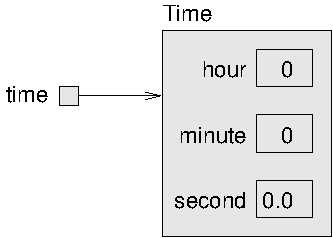
\includegraphics{figs/time.pdf}
\end{center}

%\subsection{Public vs private}

The keyword \java{public} means that a variable (or method or class) can be accessed from other classes.
The alternative is \java{private}, which means it can only be accessed inside the class where it is defined.
To prevent yourself and others from making mistakes, it's good practice to make instance variables \java{private}.

\index{data encapsulation}

If you attempt to read or write a \java{private} variable from another class, you will get a compiler error.
Private methods and instance variables are language features that help programmers ensure {\bf data encapsulation}, which means that objects in one class are isolated from other classes.
%Limiting interactions between classes is a standard technique for managing complexity.

%We can create {\bf accessor methods} like \java{getHour}, \java{getMinute}, and \java{getSecond}.
%, but it provides no methods that modify the instance variables.
%In effect, \java{Location} objects are immutable, which means that they can be shared without worrying about unexpected behavior due to aliasing.

%Making methods private helps keep the API simple.
%Classes often include helper methods that are used to implement other methods, but making those methods part of the public API might be unnecessary and error-prone.


\section{Constructors}

\index{constructor}
\index{method!constructor}
\index{static}

After declaring the instance variables, the next step is to define a constructor for the new class.
Constructors initialize the instance variables.
The syntax for constructors is similar to that of other methods, with a few exceptions:

\begin{itemize}
\item The name of the constructor is the same as the name of the class.
\item Constructors have no return type (and no return value).
\item The keyword \java{static} is omitted.
\end{itemize}

Here is an example for the \java{Time} class:

\begin{code}
    public Time() {
        this.hour = 0;
        this.minute = 0;
        this.second = 0.0;
    }
\end{code}

Where you would expect to see a return type, between \java{public} and \java{Time}, there is nothing.
That's how we (and the compiler) can tell it's a constructor as opposed to a \java{void} method.
This constructor does not take any arguments.
Each line of the constructor initializes an instance variable to zero (which in this example means midnight).

\index{this}

The variable \java{this} is a special keyword that refers to the object that we are creating.
You can use \java{this} the same way you use the name of any other object.
For example, you can read and write the instance variables of \java{this}, and you can pass \java{this} as an argument to other methods.
But you do not declare \java{this}, and you can't make an assignment to it.

A common error when writing constructors is to put a \java{return} statement at the end.
Like \java{void} methods, constructors do not return values.
Another mistake that beginning programmers make is to invoke the \java{new} operation inside the constructor.
For example, writing the code \java{new Time(0, 0, 0.0)} in the constructor results in infinite recursion.

%\subsection{More constructors}

\index{overloading}

Constructors can be overloaded, just like other methods, which means that you can provide multiple constructors with different parameters.
Java knows which constructor to invoke by matching the arguments after \java{new} with the parameters of the constructors.

For example, it is common to have one constructor that takes no arguments (the ``default constructor'') and another one that takes a parameter list identical to the list of instance variables (the ``explicit value constructor'').

\begin{code}
    public Time(int hour, int minute, double second) {
        this.hour = hour;
        this.minute = minute;
        this.second = second;
    }
\end{code}

Notice how the names and types of the parameters are the same as the names and types of the instance variables.
All the constructor does is copy the information from the parameters into the instance variables.

If you look at the documentation for \java{Point} and \java{Rectangle}, you will see that both classes provide similar constructors.
Overloading constructors provides the flexibility to create an object first and then fill in the blanks, or to collect all the information before creating the object.

This detail might not seem very interesting, and in fact it is not.
Writing constructors is a boring, mechanical process, and some IDEs will automatically generate them for you.
You will find that you can write them quickly just by looking at the list of instance variables.


\section{Creating a new object}

\index{new}
\index{statement!new}

Although constructors look like methods, you never invoke them directly.
When you apply the \java{new} operator, the system allocates space for the object and then invokes the constructor for you.

The following program (in the \java{main} method) demonstrates two common ways to create and initialize \java{Time} objects:

\begin{code}
public class Time {
    private int hour;
    private int minute;
    private double second;

    public Time() {
        this.hour = 0;
        this.minute = 0;
        this.second = 0.0;
    }

    public Time(int hour, int minute, double second) {
        this.hour = hour;
        this.minute = minute;
        this.second = second;
    }

    public static void main(String[] args) {
        // one way to create a time object
        Time t1 = new Time();
        t1.hour = 11;
        t1.minute = 8;
        t1.second = 3.14159;
        System.out.println(t1);

        // another way to do the same thing
        Time t2 = new Time(11, 8, 3.14159);
        System.out.println(t2);
    }
}
\end{code}

The first time we apply \java{new} we provide no arguments, so Java invokes the default constructor.
The next few lines assign values to the instance variables.
The second time we invoke \java{new}, we provide arguments that match the parameters of the second constructor.
This way of initializing the instance variables is more concise and slightly more efficient.

%\section{Printing objects}
\label{printobject}

\index{print}
\index{statement!print}
\index{object!printing}

The output of this program is something like:

\begin{stdout}
Time@80cc7c0
Time@80cc807
\end{stdout}

When Java prints the value of a user-defined object type, it prints the name of the type and a hexadecimal (base 16) code that is unique for each object.
As we saw in Section~\ref{sec:system}, this code is the address of the object in memory, and it usually varies from machine to machine.
It is useful for debugging, in case you want to keep track of individual objects.

To print \java{Time} objects in a way that is more meaningful to users (as opposed to programmers), you could write a method to print the hour, minute, and second.
Using \java{printTime} in Section~\ref{time} as a starting point, we could write:

\begin{code}
    public static void printTime(Time t) {
        System.out.print(t.hour);
        System.out.print(":");
        System.out.println(t.minute);
        System.out.print(":");
        System.out.println(t.second);
    }
\end{code}

The output of this method, if we pass either \java{t1} or \java{t2} as an argument, is {\tt 11:8:3.14159}.
Although it's recognizable as a time, it's not quite in the standard format.
For example, if the number of minutes or seconds is less than 10, we expect a leading {\tt 0}.
Also, we might want to drop the decimal part of the seconds.
In other words, we want something like {\tt 11:08:03}.

Fortunately, we can use \java{printf} to format the output:

\begin{code}
    public static void printTime(Time t) {
        System.out.printf("%02d:%02d:%02.0f\n",
            t.hour, t.minute, t.second);
    }
\end{code}

As a reminder, you need to use \java{\%d} with integers and \java{\%f} with floating-point numbers.
The \java{02} option means ``two digits with leading zeros,'' and the \java{.0} option means ``zero decimal places.''
Note that \java{\%f} automatically rounds the floating-point value.


\section{The toString method}

\index{toString}
\index{method!toString}

Every object type has a method called \java{toString} that returns a string representation of the object.
When you print an object using \java{print} or \java{println}, Java invokes the object's \java{toString} method.

\index{override}

The default version of \java{toString} returns a string that contains the type of the object and its current address (see Section~\ref{printobject}).
When you define a new object type, you can {\bf override} the default behavior by providing a new method with the behavior you want.

For example, here is a \java{toString} method for \java{Time}:

\begin{code}
public String toString() {
    return String.format("%02d:%02d:%02.0f\n",
            t.hour, t.minute, t.second);
}
\end{code}

This code is essentially the same as printTime in the previous section, except that we are returning a string instead of printing it to the screen.
The \java{String.format} method works the same way as \java{printf}; in fact, the \java{printf} method invokes \java{String.format}.

You can call \java{toString} in the usual way:

\begin{code}
    Time time = new Time(11, 8, 3.14159);
    String s = time.toString();
\end{code}

Or you can invoke it indirectly through \java{println}:

\begin{code}
    System.out.println(time);
\end{code}


\section{The equals method}

\index{equals}
\index{method!equals}

When comparing objects, there are two notions of equality: objects that are {\em identical}, and objects that are {\em equivalent}.
Identical means that two variables refer to the same object.
Equivalent means that two objects have the same values.
Consider for example the following three \java{Time} variables:

\begin{code}
    Time time1 = new Time(9, 30, 0.0);
    Time time2 = time1;
    Time time3 = new Time(9, 30, 0.0);
\end{code}

Since \java{Time} is a reference type, \java{time1}, \java{time2}, and \java{time3} are references to objects.
Here is a memory diagram:

\begin{center}
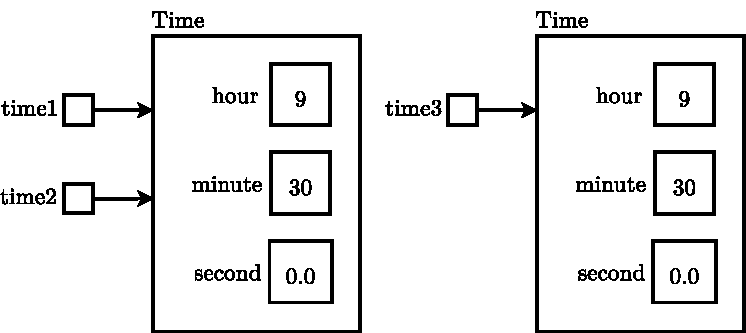
\includegraphics{figs/time2.pdf}
\end{center}

Recall that the assignment operator simply copies a reference, so \java{time1} and \java{time2} refer to the same object.
In contrast, \java{time3} points to a different object.
Whenever you apply the \java{new} operator, you create a new object in memory.

In this example, \java{time1} and \java{time2} are identical: they refer to the same object.
The \java{==} operator compares references, so \java{time1 == time2} is \java{true}.
All three variables are equivalent, since the objects they reference have the same values.
However \java{time1 == time3} is \java{false}, because their references are not the same.

There is no operator that tests equivalence, since the notion of equality is different for each type of object.
In the case of \java{Time}, we could write a method that compares hours, minutes, and seconds:

\begin{code}
    public static boolean sameTime(Time t1, Time t2) {
        return t1.hour == t2.hour
            && t1.minute == t2.minute
            && t1.second == t2.second;
    }
\end{code}

\index{instance method}

This method works just fine, but it's not the way most Java classes are designed.
Instead, objects may provide a non-\java{static} named \java{equals} that defines equality.
All we have to do is rewrite \java{sameTime} as an {\bf instance method}:

\begin{code}
    public boolean equals(Time t2) {
        return this.hour == t2.hour
            && this.minute == t2.minute
            && this.second == t2.second;
    }
\end{code}

By way of comparison, here is how each of the methods are invoked:

\begin{code}
    System.out.println(Time.sameTime(time1, time3));
    System.out.println(time1.equals(time3));
\end{code}

The latter method is certainly easier to read and understand.
Inside the \java{equals} method, the reference to \java{time1} is the current object \java{this}, and \java{time3} is the parameter \java{t2}.

Like the \java{toString} method, Java provides a default implementation of the \java{equals} method.
If you don't define your own, then \java{equals} behaves the same way as the \java{==} operator, which is often incorrect.
Unlike the \java{toString} method, \java{equals} requires a parameter: the other object you need to compare.
So in order to override the default \java{equals} method, you need to write it this way:

\begin{code}
    public boolean equals(Object obj) {
        if (!(obj instanceof Time)) {
            return false;
        }
        Time t2 = (Time) obj;
        return this.hour == t2.hour
            && this.minute == t2.minute
            && this.second == t2.second;
    }
\end{code}

Because the parameter is declared as an \java{Object}, one could in theory pass any type of data (like a \java{String} or \java{Scanner}) to this method.
The \java{instanceof} operator tests whether \java{obj} references an actual \java{Time} object.
If it passes the test, we can safely cast \java{obj} to a \java{Time} reference and perform the equality test as before.

Of course, the \java{equals} method may be arbitrarily complex.
You could design it, for example, to allow \java{Time} and \java{String} objects to be equal if they represent the same time.
However that design would likely confuse other programmers, since normally objects are only considered equal if they are of the same type.


\section{The compareTo method}

%\index{pure function}
%\index{method!pure function}
%, and it has no side effects like modifying an argument or printing something.
%The only result of invoking a pure function is the return value.

In contrast to instance methods, \java{static} methods do not refer to a specific object.
The result of a \java{static} method depends only on the arguments.
For example, \java{isAfter} compares two \java{Time}s and returns a \java{boolean} that indicates whether the first operand comes after the second:

\begin{code}
    public static boolean isAfter(Time time1, Time time2) {
        if (time1.hour < time2.hour) return false;
        if (time1.hour > time2.hour) return true;

        if (time1.minute < time2.minute) return false;
        if (time1.minute > time2.minute) return true;

        if (time1.second < time2.second) return false;
        return true;
    }
\end{code}

What is the result of this method if the two times are equal?
Does that seem like the appropriate result for this method?
If you were writing the documentation for this method, would you mention that case specifically?

A better solution would be to define a \java{compareTo} method.
We have already seen how to compare two strings in this way: \java{time1.compareTo(time2)}.

\begin{code}
    public int compareTo(Time t2) {
        if (this.hour < t2.hour) return -1;
        if (this.hour > t2.hour) return +1;
        
        if (this.minute < t2.minute) return -1;
        if (this.minute > t2.minute) return +1;
        
        if (this.second < t2.second) return -1;
        if (this.second > t2.second) return +1;
        
        return 0;
    }
\end{code}

If \java{this} time comes before the other time, then compareTo returns \java{-1}.
It returns \java{+1} when \java{this} time comes after the other time.
If both times are the same (in the \java{equals} sense), \java{compareTo} returns \java{0}.


\section{Adding times}

Throughout the chapter, we have demonstrated how \java{static} methods can and should be implemented as instance methods.
As a further example, \java{addTime} calculates the sum of two times.
Here is a rough draft of a method that is not quite right.

\begin{code}
    public static Time addTime(Time t1, Time t2) {
        Time sum = new Time();
        sum.hour = t1.hour + t2.hour;
        sum.minute = t1.minute + t2.minute;
        sum.second = t1.second + t2.second;
        return sum;
    }
\end{code}

%Note that although this method returns a \java{Time} object, it is not a constructor.
%You should go back and compare the syntax of a method like this with the syntax of a constructor, because it is easy to get confused.

%Here is an example of how to use this method.
If it is {\tt 9:14:30}, and your bread maker takes 3 hours and 35 minutes, you could use \java{addTime} to figure out when the bread will be done.
%Since \java{currentTime} contains the current time and \java{breadTime} contains the amount of time it takes for your bread maker to make bread, we can use \java{addTime} to figure out when the bread will be done.

\begin{code}
    Time currentTime = new Time(9, 14, 30.0);
    Time breadTime = new Time(3, 35, 0.0);
    Time doneTime = addTime(currentTime, breadTime);
\end{code}

We can rewrite \java{addTime} as an instance method by deleting the word \java{static} and removing the first parameter.

\begin{code}
    public Time addTime(Time t2) {
        Time sum = new Time();
        sum.hour = this.hour + t2.hour;
        sum.minute = this.minute + t2.minute;
        sum.second = this.second + t2.second;
        return sum;
    }
\end{code}

When calling this version of \java{addTime}, we still need to specify the \java{currentTime} object.
Because of the dot operator, it becomes \java{this} in the method.

\begin{code}
    Time doneTime = currentTime.addTime(breadTime);
\end{code}

The result of this method is {\tt 12:49:30.0}, which is correct.
On the other hand, there are cases where the result is not correct.
The problem is that this method does not deal with cases where the number of seconds or minutes adds up to more than 60.
In that case, we have to ``carry'' the extra seconds into the minutes column, or extra minutes into the hours column.

\begin{code}
    public Time addTime(Time t2) {
        Time sum = new Time();
        sum.hour = this.hour + t2.hour;
        sum.minute = this.minute + t2.minute;
        sum.second = this.second + t2.second;

        if (sum.second >= 60.0) {
            sum.second -= 60.0;
            sum.minute += 1;
        }
        if (sum.minute >= 60) {
            sum.minute -= 60;
            sum.hour += 1;
        }
        return sum;
    }
\end{code}

\index{increment}
\index{decrement}
\index{operator!increment}
\index{operator!decrement}

This code demonstrates two operators we have not seen before, \java{+=} and \java{-=}.
These operators provide a concise way to increment and decrement variables.
They are similar to \java{++} and \java{--}, except (1) they work on \java{double}s as well as \java{int}s, and (2) the amount of the increment does not have to be 1.
The statement \java{sum.second -= 60.0;} is equivalent to \java{sum.second = sum.second - 60;}


\section{Accessors and mutators}

\index{immutable}

Notice how the \java{addTime} method does not change \java{this} object.
Instead, it creates a \java{new} object to store the results.
All of the \java{String} methods work the same way.
Up to this point, we have designed \java{Time} to be immutable.

\index{accessor}
\index{method!accessor}

Because \java{hour}, \java{minute}, and \java{second} are \java{private}, there is no way for outside classes to access them directly.
The only method we have provided for other to look at the time is \java{toString}.
As a convenience, we can also write \java{public} {\bf accessor} methods that return a copy of the \java{private} values.

\begin{code}
    public int getHour() {
        return hour;
    }

    public int getMinute() {
        return minute;
    }

    public int getSecond() {
        return second;
    }
\end{code}

\index{mutator}
\index{method!mutator}

If we want the class to be immutable, we would stop here and have a complete implementation.
But if we want other programmers (including ourselves) to be able to change the time from other classes, we should also provide the corresponding {\bf mutator} methods.

\begin{code}
    public void setHour(int hour) {
        this.hour = hour;
    }

    public void setMinute(int minute) {
        this.minute = minute;
    }

    public void setSecond(int second) {
        this.second = second;
    }
\end{code}

Accessors and mutators are the formal terms for referring to these types of methods, but many programmers simply call them getters and setters.
These methods are intentionally simple, and many IDEs will generate them for you automatically with a press of a button.
The absence or presence of these methods allows the class designer to control how the object's data is used from the outside.

Mutator methods are often one line of code, but they don't have to be.
As another example of a mutator, consider \java{increment}, which adds a given number of seconds to a \java{Time} object.
Again, a rough draft of this method looks like:

\begin{code}
    public void increment(double secs) {
        this.second += secs;
        if (this.second >= 60.0) {
            this.second -= 60.0;
            this.minute += 1;
        }
        if (this.minute >= 60) {
            this.minute -= 60;
            this.hour += 1;
        }
    }
\end{code}

The first line performs the basic operation; the remainder deals with the same cases we saw before.

What happens if the argument \java{secs} is much greater than 60?
In that case, it may not be enough to subtract 60 once; we have to keep doing it until \java{second} is below 60.
We can do that by replacing the \java{if} statements with \java{while} statements:

\begin{code}
    public void increment(double secs) {
        this.second += secs;
        while (this.second >= 60.0) {
            this.second -= 60.0;
            this.minute += 1;
        }
        while (this.minute >= 60) {
            this.minute -= 60;
            this.hour += 1;
        }
    }
\end{code}

This solution is correct, but it's not very efficient.
Can you think of a solution that does not require iteration?


\section{Vocabulary}

\begin{description}

\term{class}
Previously, we defined a class as a collection of related methods.
Now you know that a class is also a template for a new type of object.

\term{instance}
A member of a class.
Every object is an instance of some class.

\term{constructor}
A special method that initializes the instance variables of a newly-constructed object.

\term{instance variables}
The attributes of an object; non-\java{static} variables defined at the class level.

\term{data encapsulation}
A technique for bundling multiple named variables into a single object.

\term{override}
Replacing a default implementation of a method, such as \java{equals} or \java{toString}.

\term{instance methods}
Non-\java{static} methods that have access to \java{this} and the instance variables.

\term{accessor}
A method that returns a copy of a \java{private} variable.

\term{mutator}
A method that changes one or more of the objects it receives as parameters.
It is usually \java{void} and modifies \java{this}.

\end{description}


\section{Exercises}


\begin{exercise}
In the board game Scrabble\footnote{Scrabble is a registered trademark owned in the U.S.A and Canada by Hasbro Inc., and in the rest of the world by J.W. Spear \& Sons Limited of Maidenhead, Berkshire, England, a subsidiary of Mattel Inc.}, each tile contains a letter, which is used to spell words in rows and columns, and a score, which is used to determine the value of words.

\begin{enumerate}

\item Write a definition for a class named \java{Tile} that represents Scrabble tiles.
The instance variables should be a character named \java{letter} and an integer named \java{value}.

\item Write a constructor that takes parameters named \java{letter} and \java{value} and initializes the instance variables.

\item Write a method named \java{printTile} that takes a \java{Tile} object as a parameter and prints the instance variables in a reader-friendly format.

\item Write a method named \java{testTile} that creates a Tile object with the letter \java{Z} and the value 10, and then uses \java{printTile} to print the state of the object.

\item Implement the \java{toString} and \java{equals} methods for a \java{Tile}.

\item Create accessors and mutators for each of the attributes.

\end{enumerate}

The point of this exercise is to practice the mechanical part of creating a new class definition and code that tests it.
\end{exercise}


\begin{exercise}
Write a class definition for \java{Date}, an object type that contains three integers: \java{year}, \java{month}, and \java{day}.
This class should provide two constructors.
The first should take no parameters and initialize a default date.
The second should take parameters named \java{year}, \java{month} and \java{day} and use them to initialize the instance variables.

Write a \java{main} method that creates a new \java{Date} object named \java{birthday}.
The new object should contain your birth date.
You can use either constructor.
Compare your implementation to \java{java.util.Date}.
\end{exercise}


\begin{exercise}
\label{ex.rational}

A rational number is a number that can be represented as the ratio of two integers.
For example, $2/3$ is a rational number, and you can think of 7 as a rational number with an implicit 1 in the denominator.
For this assignment, you are going to write a class definition for rational numbers.

\begin{enumerate}

\item Create a new program called \java{Rational.java} that defines a class named \java{Rational}.
A \java{Rational} object should have two integer instance variables to store the numerator and denominator.

\item Write a constructor that takes no arguments and that sets the numerator to 0 and denominator to 1.

\item Write a method called \java{printRational} that takes a Rational object as an argument and prints it in some reasonable format.

\item Write a \java{main} method that creates a new object with type Rational, sets its instance variables to some values, and prints the object.

\item At this stage, you have a minimal testable program.
Test it and, if necessary, debug it.

\item Write a second constructor for your class that takes two arguments and that uses them to initialize the instance variables.

\item Write a method called \java{negate} that reverses the sign of a rational number.
This method should be a modifier, so it should be \java{void}.
Add lines to \java{main} to test the new method.

\item Write a method called \java{invert} that inverts the number by swapping the numerator and denominator.
Add lines to \java{main} to test the new method.

\item Write a method called \java{toDouble} that converts the rational number to a double (floating-point number) and returns the result.
This method is a pure function; it does not modify the object.
As always, test the new method.

\item Write a modifier named \java{reduce} that reduces a rational number to its lowest terms by finding the greatest common divisor (GCD) of the numerator and denominator and dividing through.
This method should be a pure function; it should not modify the instance variables of the object on which it is invoked.
To find the GCD, see Exercise~\ref{gcd}).

\item Write a method called \java{add} that takes two Rational numbers as arguments and returns a new Rational object.
The return object should contain the sum of the arguments.

\item There are several ways to add fractions.
You can use any one you want, but you should make sure that the result of the operation is reduced so that the numerator and denominator have no common divisor (other than 1).
\end{enumerate}

The purpose of this exercise is to write a class definition that includes a variety of methods, including constructors, accessors, mutators, \java{static} methods, and instance methods.
\end{exercise}


\end{document}
